% Software Development for Mobile Devices
\documentclass[11pt,english,numbers=endperiod,parskip=half]{scrartcl}

\usepackage{color}
\usepackage{graphicx}
\usepackage{minted}
\usepackage{fancyhdr}
\usepackage{pdflscape}

\pagestyle{fancy}

\rhead{Daniel Parker - 971328X}
\lhead{COS30017 - Software Development for Mobile Devices}

\title{Assignment 05}
\subtitle{COS30017 - Software Development for Mobile Devices}
\author{Daniel Parker 971328X}

\date{\today}

\begin{document}
\maketitle
\thispagestyle{empty}

\section{Task 1}
\subsection{App Wiring}
The app uses two activities, one to display a list of locations (loaded from file),
and another to show the specific sun rise and set times for that location. The
second activity is passed a \textit{Location} object as context for showing the
correct times for the selected location. The following code snippets show the
specific `wiring' components, such as intents and ListAdapters that are required,
as boilerplate code to make this app function as intended.

\textbf{LocationsActivity: }Responsible for the listview landing activity and
how that is initialised with Location data. This activity extends the abstract
\textit{ListActivity} class to allow for list item select event overriding. This
Activity also creates intents to start the \textit{SuntimeActivity} and show a
particular locations sun times.

\textbf{LocationsAdapter: }Responsible for converting the underlying Location
data model from it's object form into the UI views. This is set as the list
adapter in the \textit{LocationsActivity} class.

\textbf{SuntimeActivity: }Responsible for displaying a given location's sun times.
This class makes use of some calculation classes; \textit{AstronomicalCalendar},
\textit{GeoLocation}, and \textit{SunTimesCalculator}. Those classes were supplied,
therefor I will not be including code snippets from them.

\textbf{Location: }This is the data model for a location that is shared between
the list adapter and the \textit{SuntimeActivity} class. Objects of this class
are \textit{Parcelable} so that they can be passed as extra data in intents that
are created by the list activity for \textit{SuntimeActivity}.


% Source code needs landscape
\begin{landscape}

\subsubsection{LocationsActivity}
\inputminted[firstline=25, lastline=62]{java}{../../Apps/Suntime/app/src/main/java/au/net/danielparker/suntime/ui/LocationsActivity.java}

\subsubsection{LocationsAdapter}
\inputminted[firstline=16, lastline=38]{java}{../../Apps/Suntime/app/src/main/java/au/net/danielparker/suntime/ui/LocationsAdapter.java}

\subsubsection{SuntimeActivity}
\inputminted[firstline=21, lastline=80]{java}{../../Apps/Suntime/app/src/main/java/au/net/danielparker/suntime/ui/SuntimeActivity.java}

\subsubsection{Location}
\inputminted[firstline=15, lastline=71]{java}{../../Apps/Suntime/app/src/main/java/au/net/danielparker/suntime/models/Location.java}

\subsection{Custom Locations}
\inputminted[firstline=1, lastline=2]{text}{../../Apps/Suntime/app/src/main/assets/au_locations.txt}

\end{landscape}



\subsection{Screenshots}
\setlength\fboxsep{0pt}
\setlength\fboxrule{0.5pt}

\begin{figure}[H]
\centering{
	\fbox{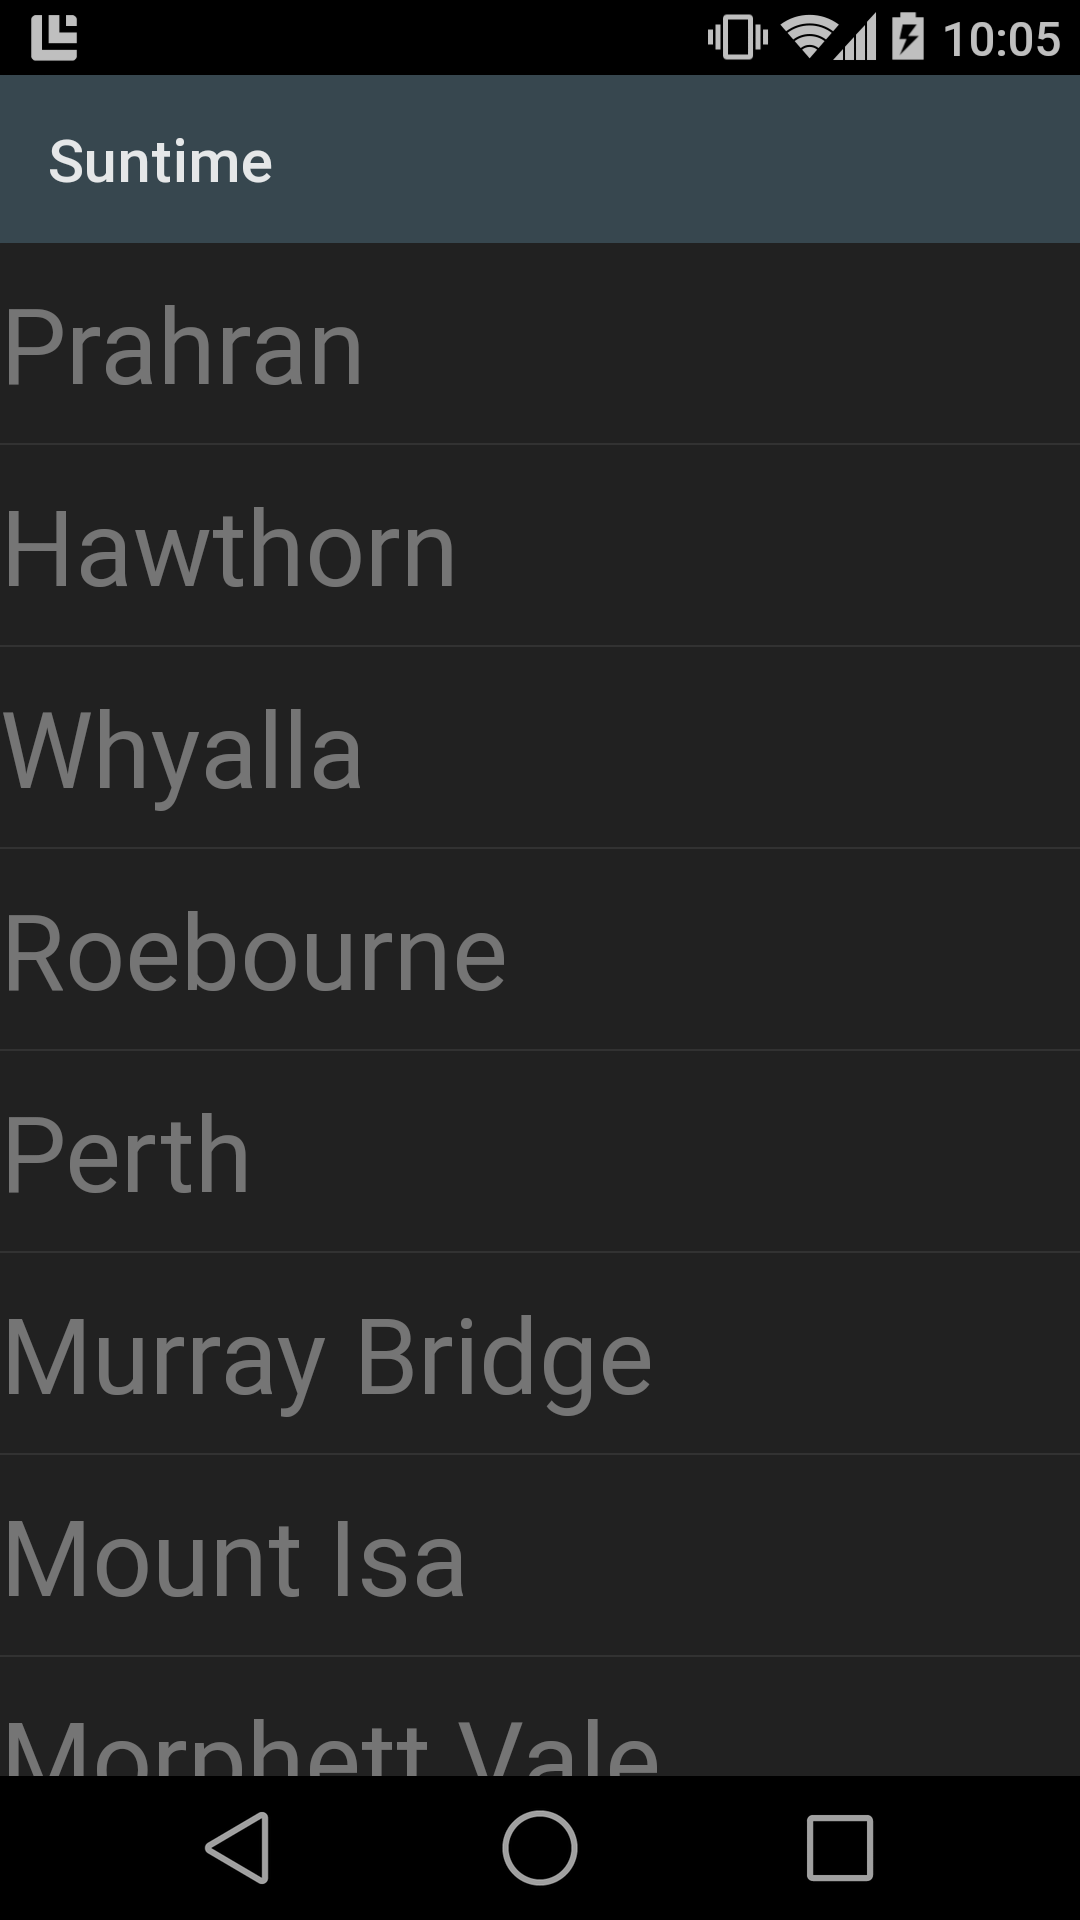
\includegraphics[width=5cm]{images/list.png}}
}\\
\end{figure}
\bigskip

\begin{figure}[H]
\centering{
	\fbox{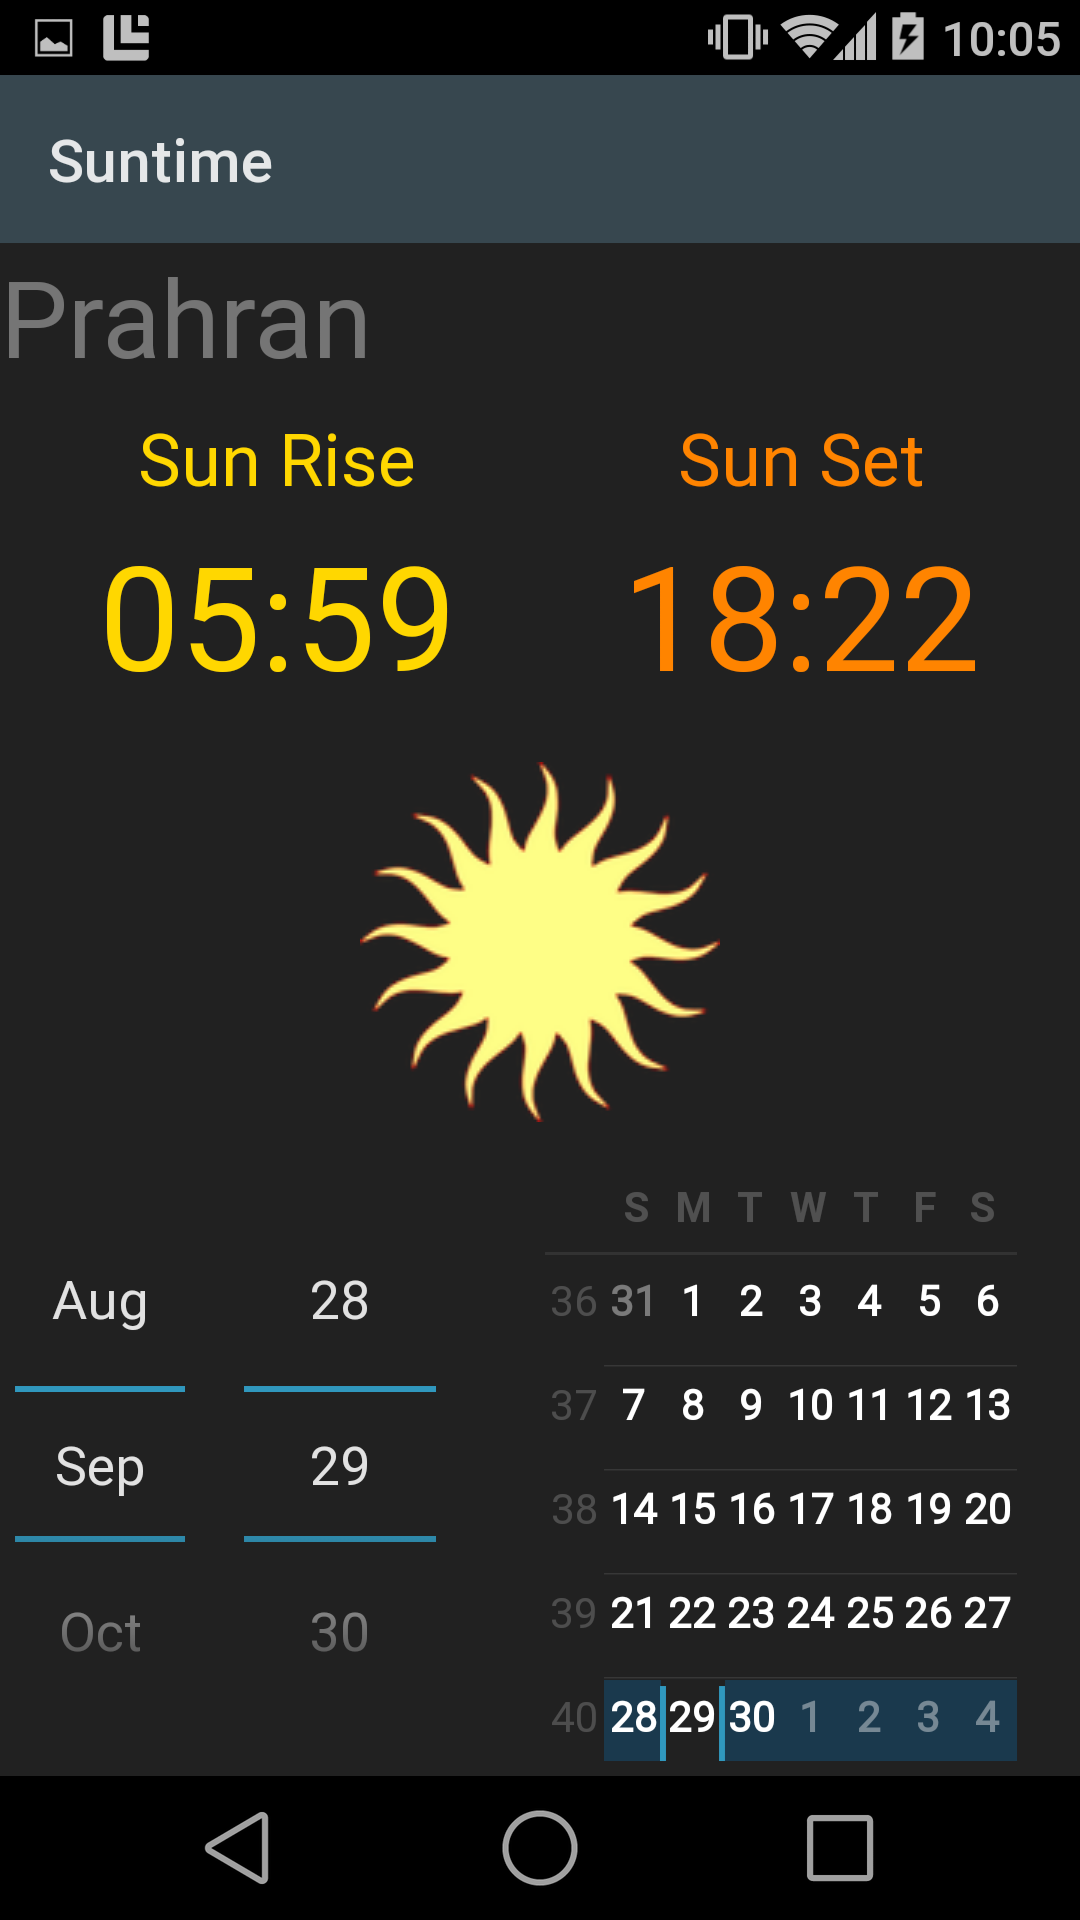
\includegraphics[width=5cm]{images/prahran.png}}
}\\
\end{figure}
\bigskip

\begin{figure}[H]
\centering{
	\fbox{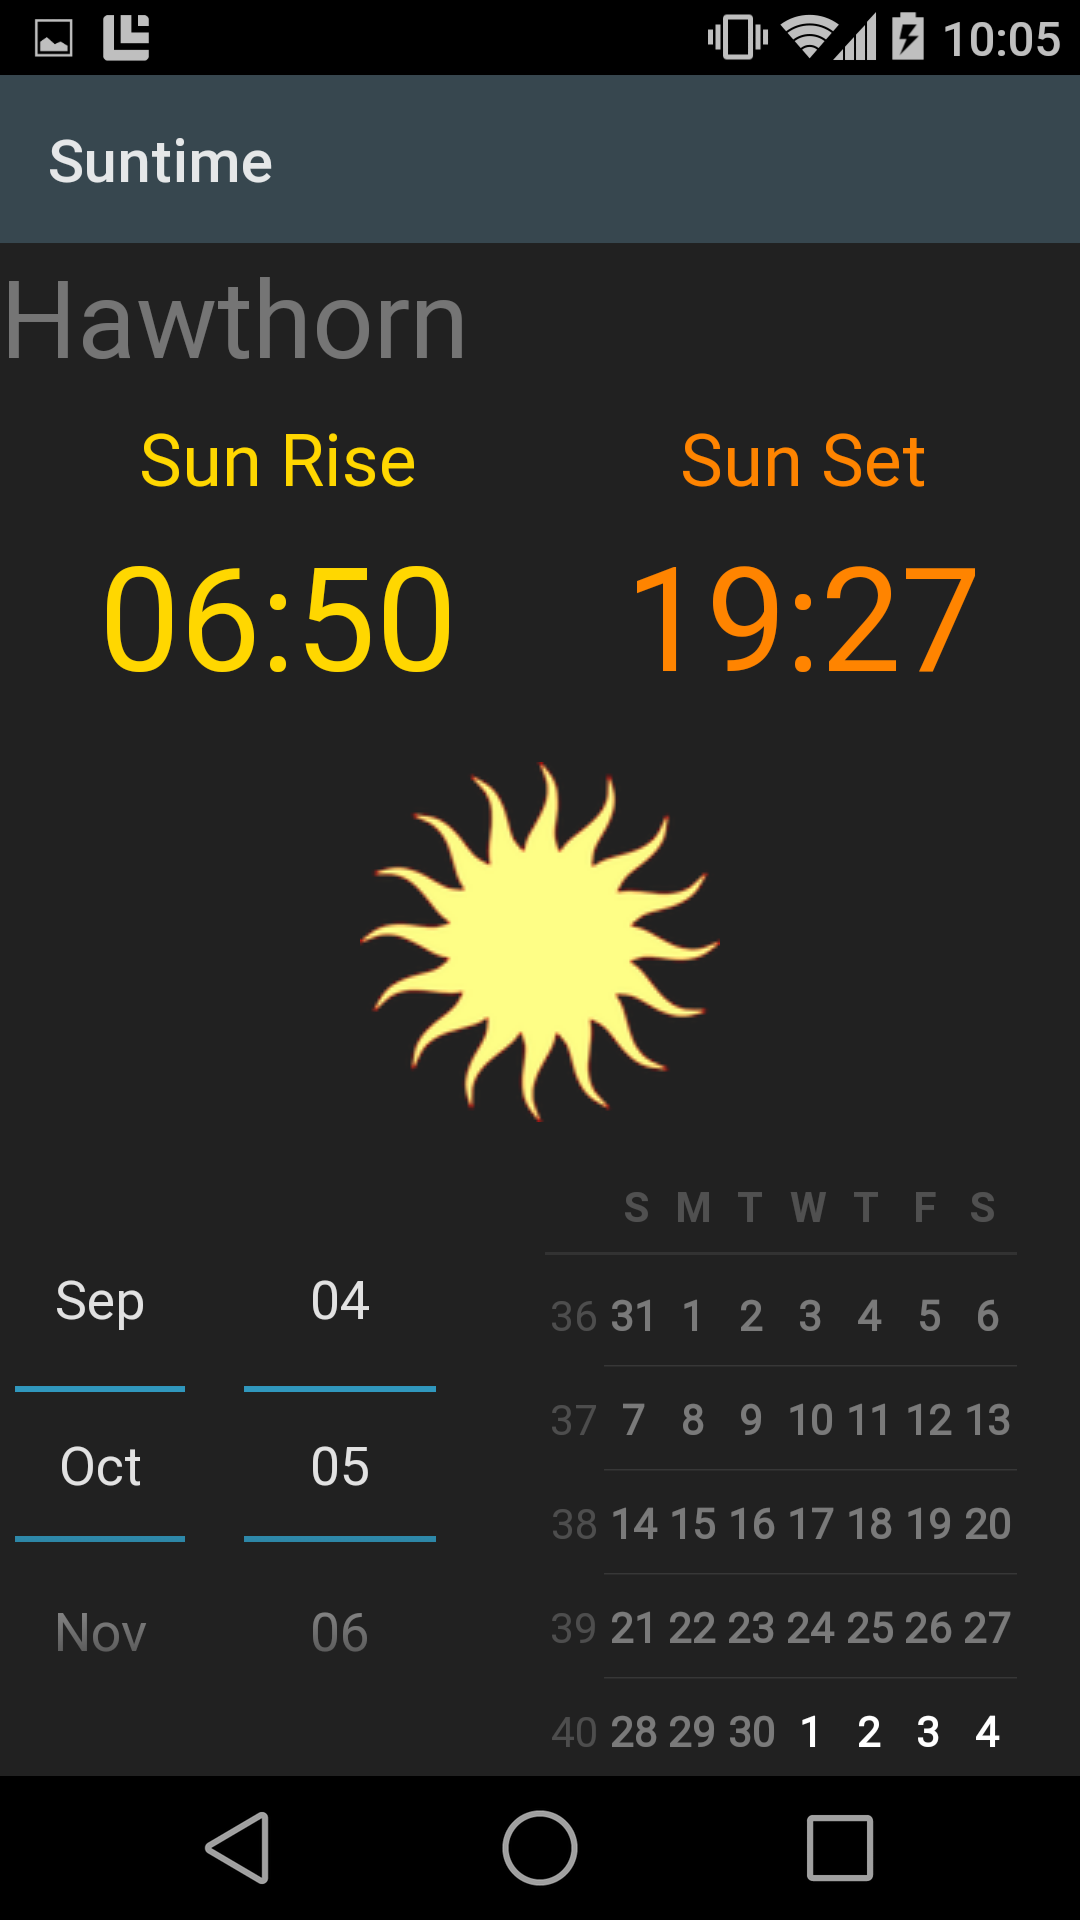
\includegraphics[width=5cm]{images/hawthorn.png}}
}\\
\end{figure}
\bigskip

\section{Task 2}
\subsection{User Stories}
\begin{enumerate}
	\item{As a recreational road-cyclist, I want to get the sun rise time and
	weather conditions so that I can maximise the time riding in daylight before
	I go to work.}
	\item{As an adventure tour guide, I want to know the sun set times for a
	period of a week so that my group of campers can have their tents set up
	before sundown.}
	\item{As a group runner, I want to be able to share the sun rise time with
	those that I'm running with so that we can all be ready to run as soon as
	there's daylight.}
	\item{As a zookeeper, I need to know the sun rise times so that I can plan
	to clean the animal enclosures and feed the animals before the zoo opens.}
\end{enumerate}
\subsection{User Stories vs. Scenarios}
When comparing user stories and scenarios as a way of showing how an application
 may be used, I think it user stories are better to use, due to the fact that
they are shorter and tend to only focus on one specific feature. The Scenarios
have a lot of information, and potentially every single feature can be listed as
 part of the scenario story. This leads tohaving to go thoroughly through the
scenarios to actually get the important information out.
\subsection{Prototype}
\subsubsection{Screenshots}
\begin{figure}[H]
\centering{
	\fbox{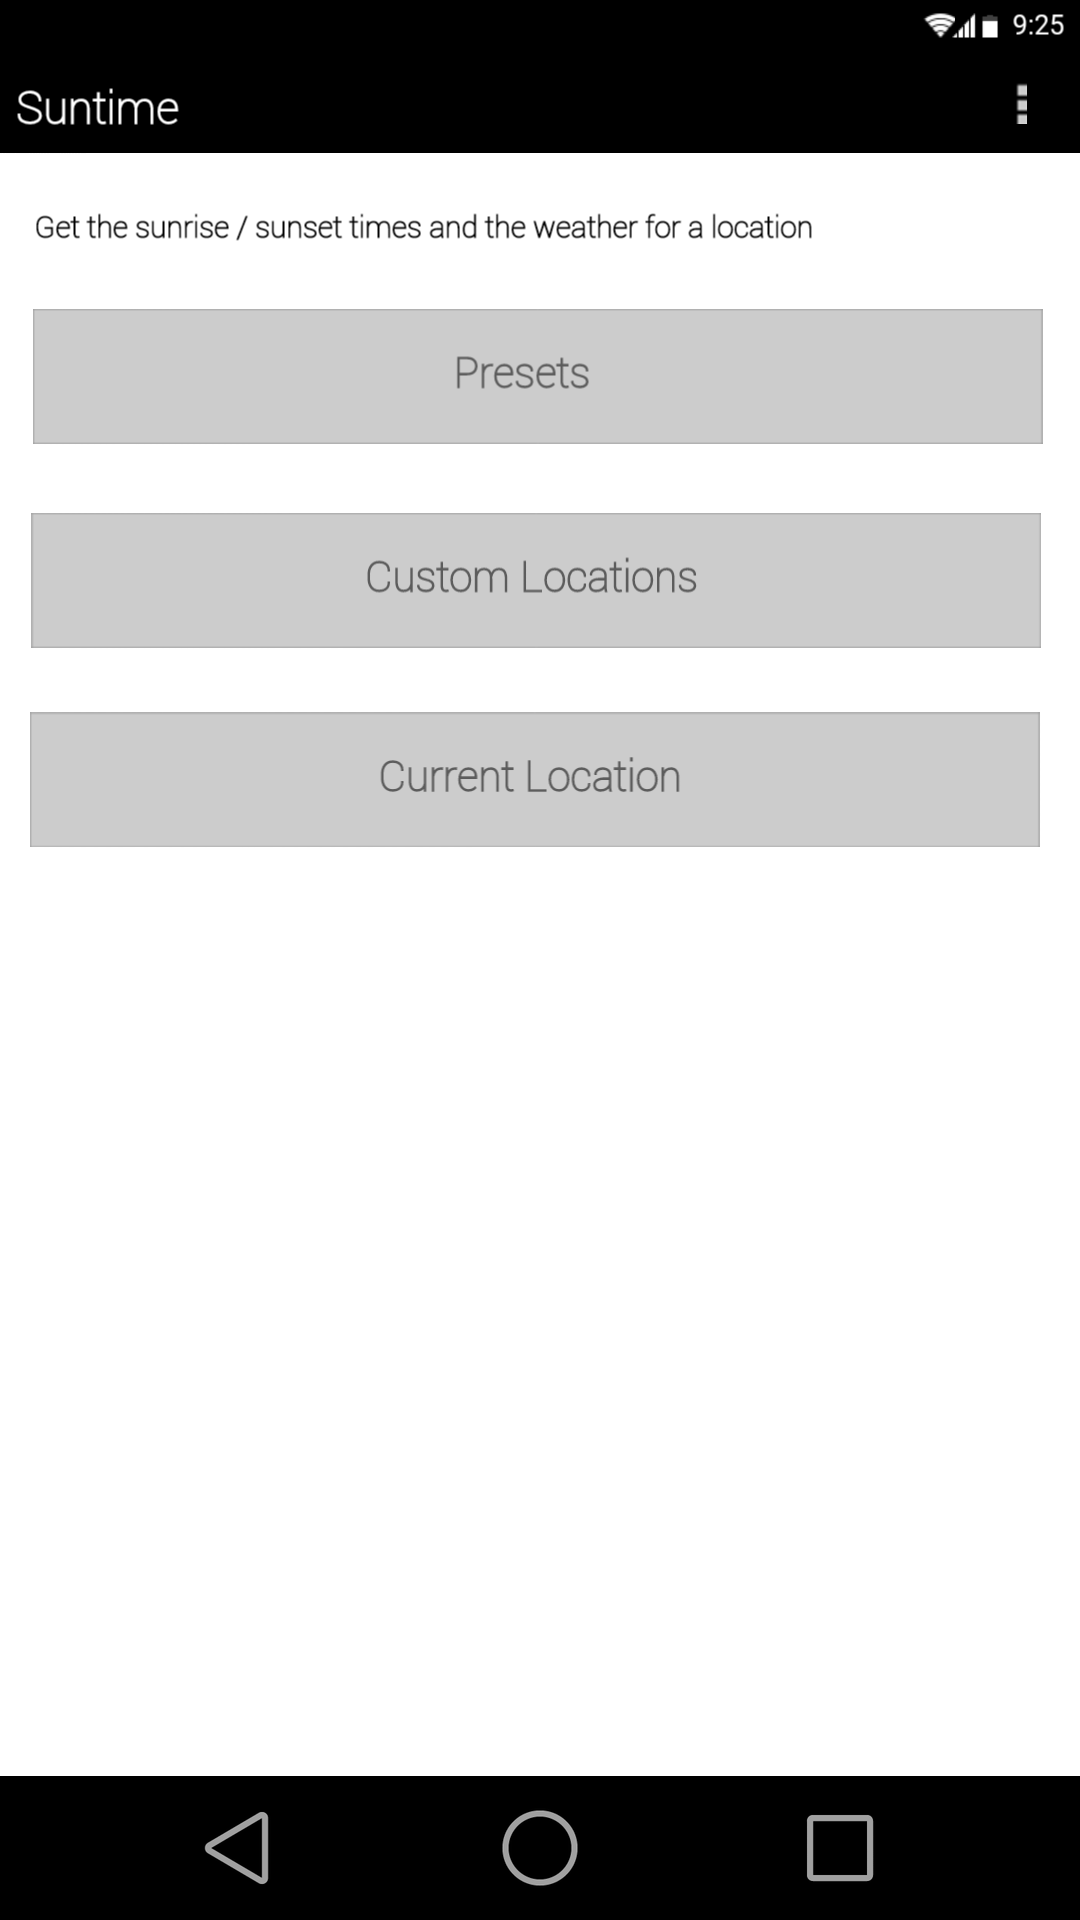
\includegraphics[width=5cm]{images/home.png}}
	\caption{HOME}
}
\end{figure}
\bigskip
\textbf{Description: }This is the first screen the user will see.
The user has three options for selecting a location;
\textit{Presets}, \textit{Custom Locations}, and \textit{Current Location}.

\textbf{Features: }Options for locations as described above. Can detect current
location as an option.

\begin{figure}[H]
\centering{
	\fbox{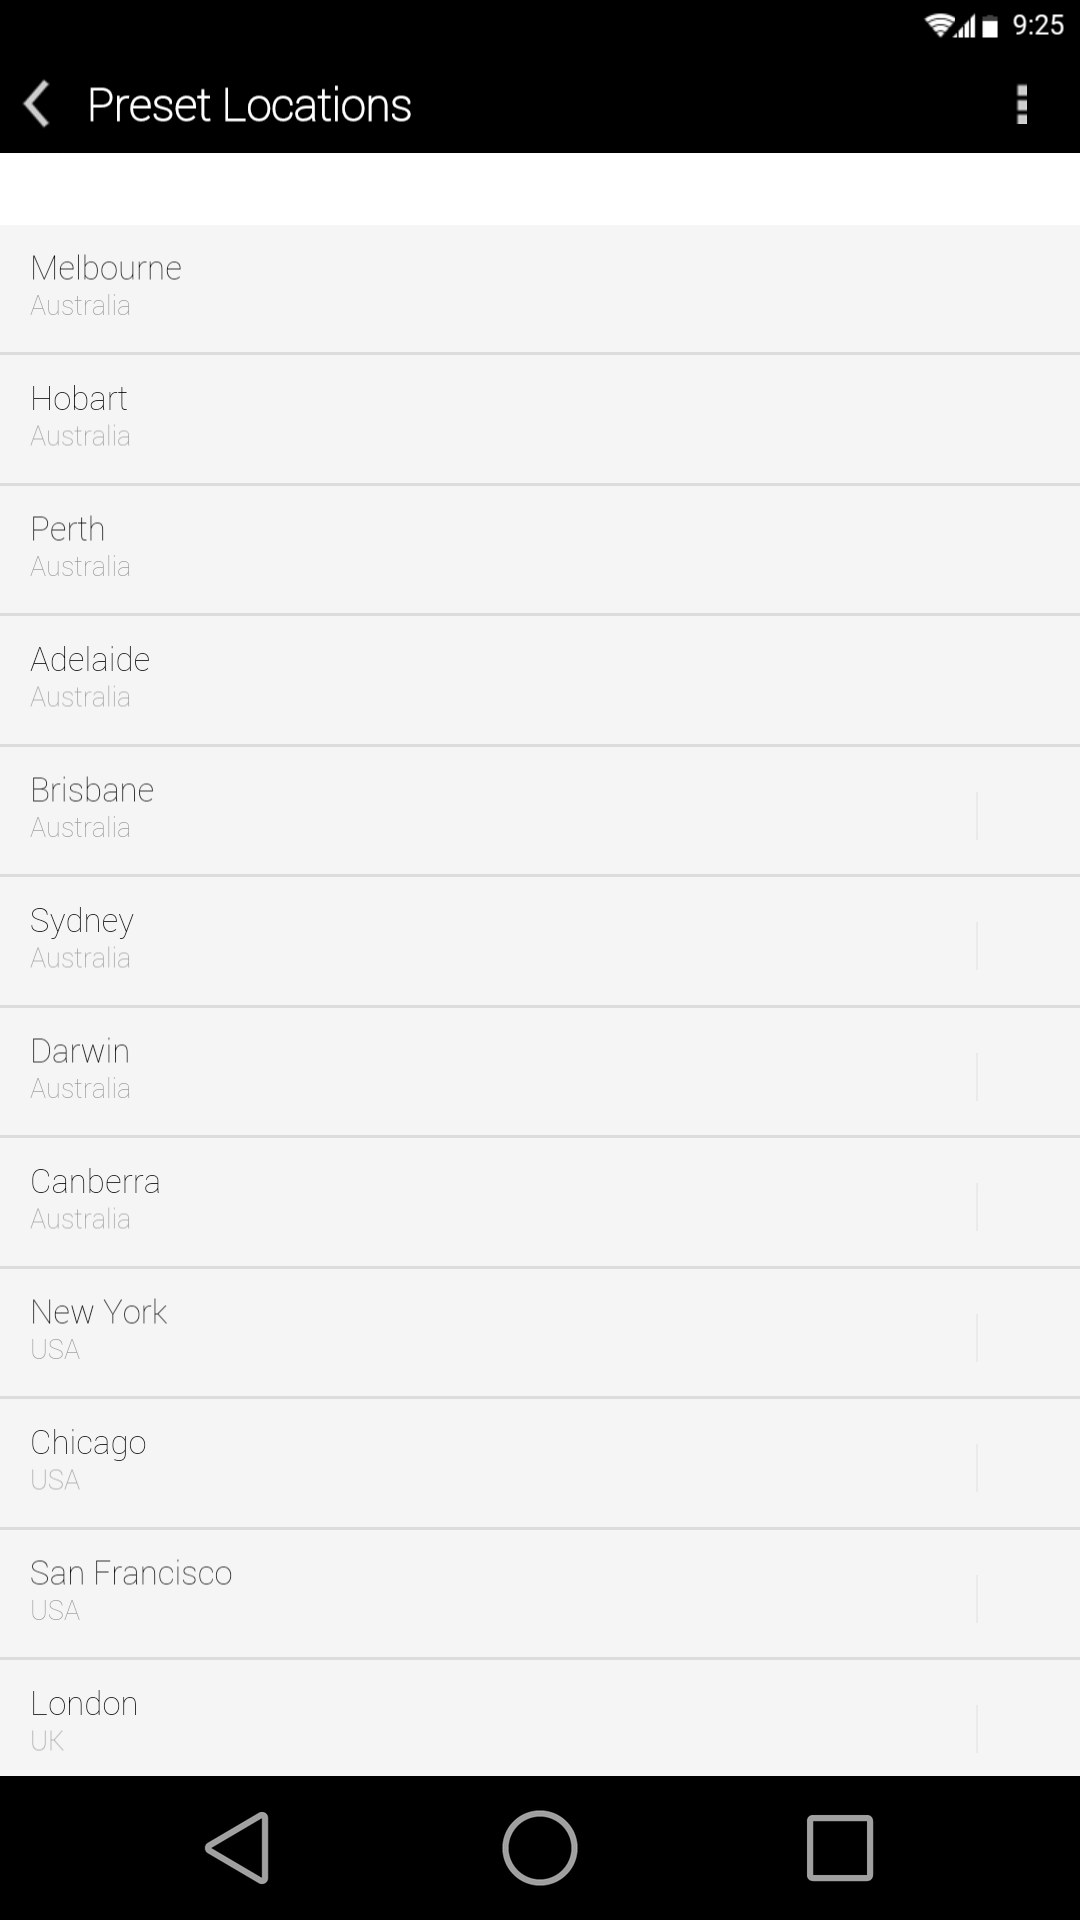
\includegraphics[width=5cm]{images/presets.png}}
	\caption{PRESETS}
}
\end{figure}
\bigskip
\textbf{Description: }The user can select one of the preset locations from this
list and they will then be taken to select a date / date range.

\textbf{Features: }Select from pre-built set of locations.

\begin{figure}[H]
\centering{
	\fbox{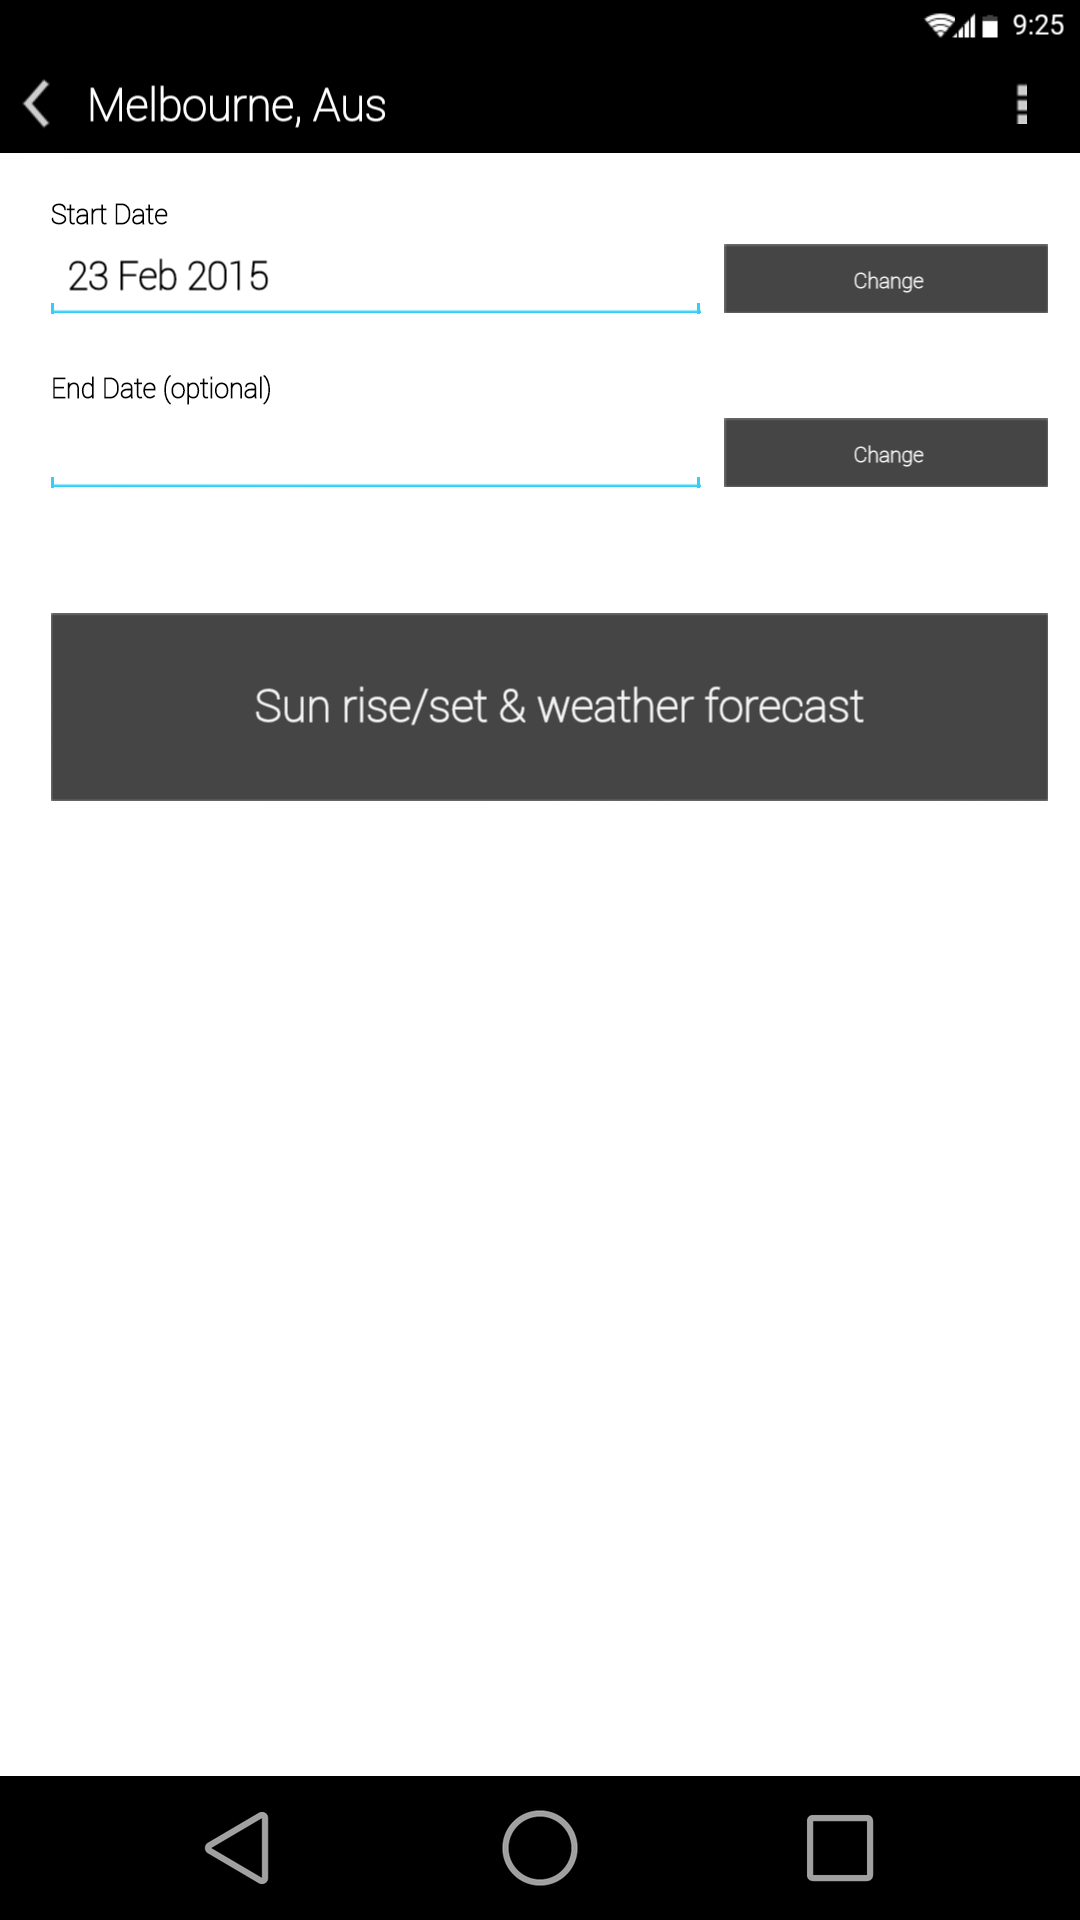
\includegraphics[width=5cm]{images/date-single.png}}
	\caption{DATE-SELECT}
}
\end{figure}
\bigskip
\textbf{Description: }User can select a single date or date range to view the
sun rise/set and weather. A different view is shown to them depending on whether
a single date or a range is selected.

\textbf{Features: }Select a date or a date range to view sun times and weather forecast.

\begin{figure}[H]
\centering{
	\fbox{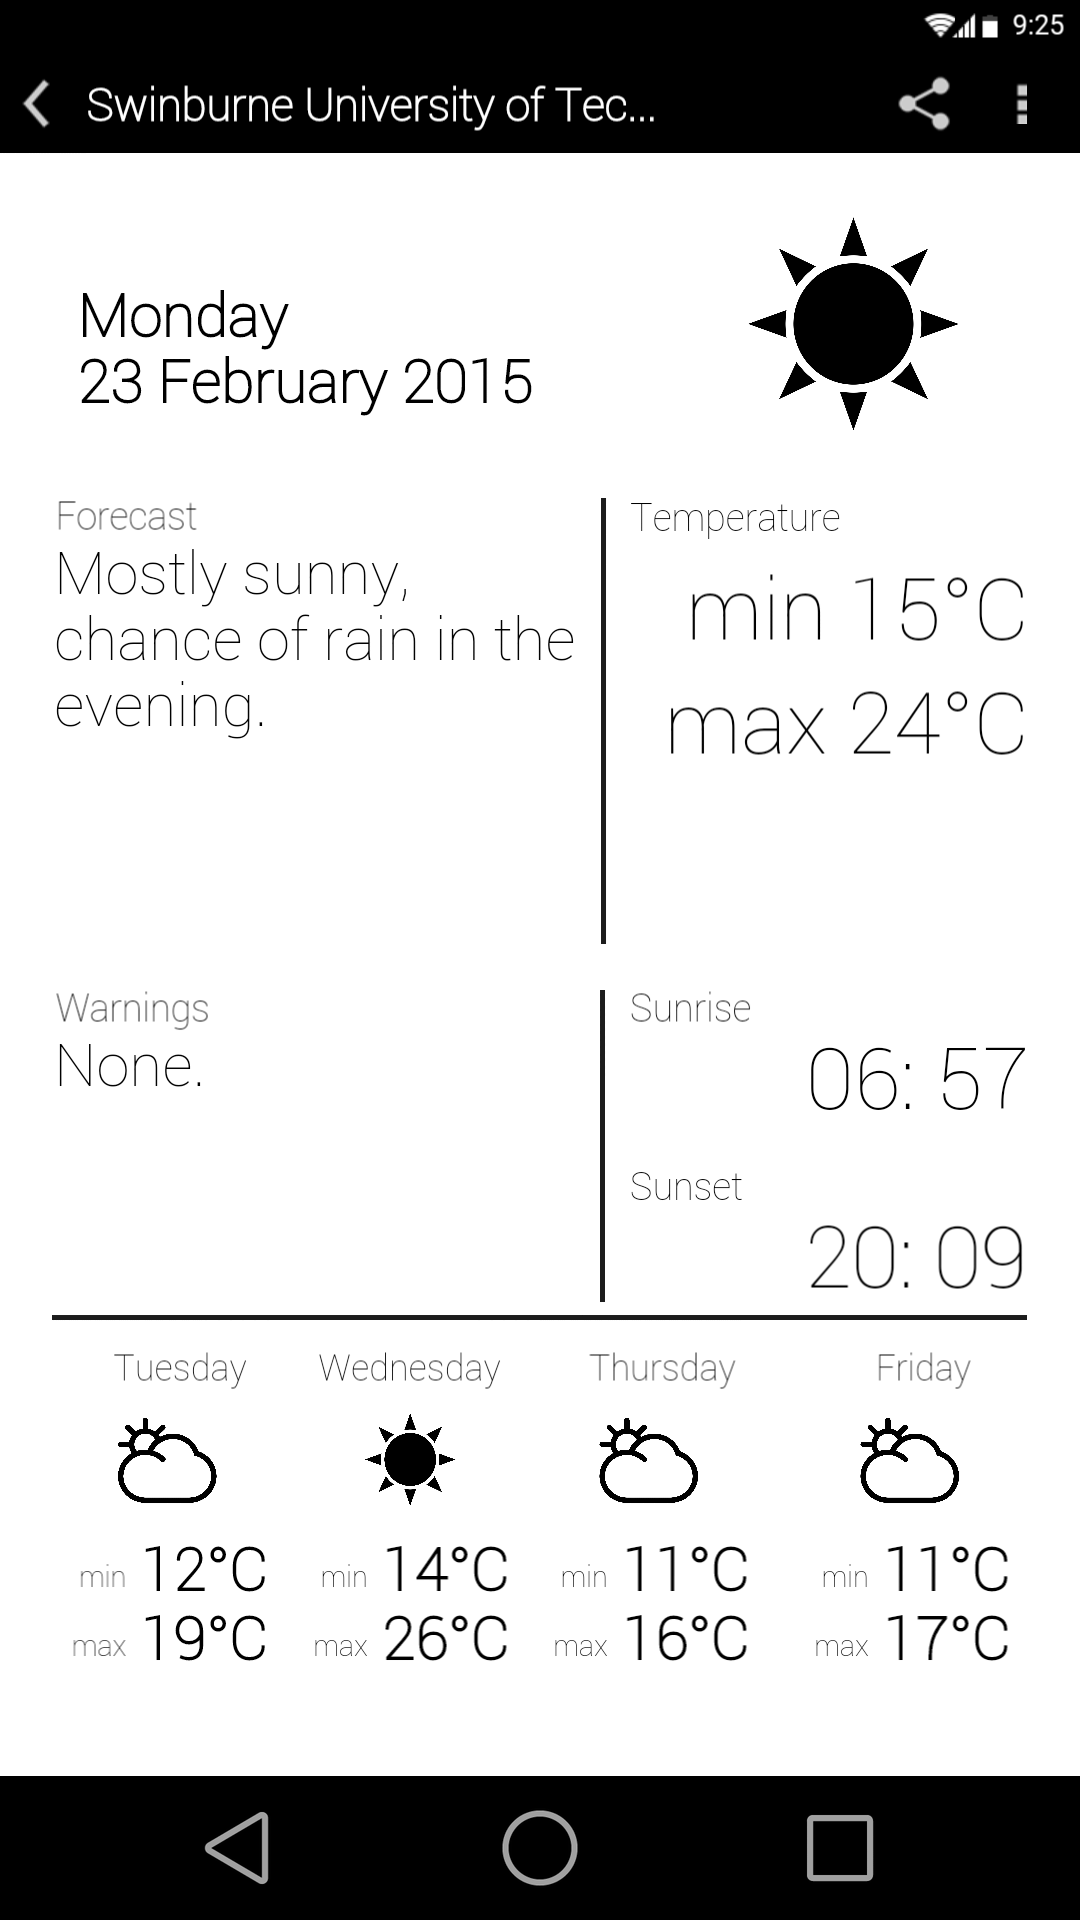
\includegraphics[width=5cm]{images/weather.png}}
	\caption{SUN-WEATHER}
}
\end{figure}
\bigskip
\textbf{Description: }This screen shows the weather and sun rise/set times for
the selected date. The weather for the next 4 days is also shown. User can share
this information by pressing the share icon in the action bar.

\textbf{Features: }Show sun rise/set times for date/location. Share information
via SMS and email (or any other app). View weather forecast (current, and near future).

\begin{figure}[H]
\centering{
	\fbox{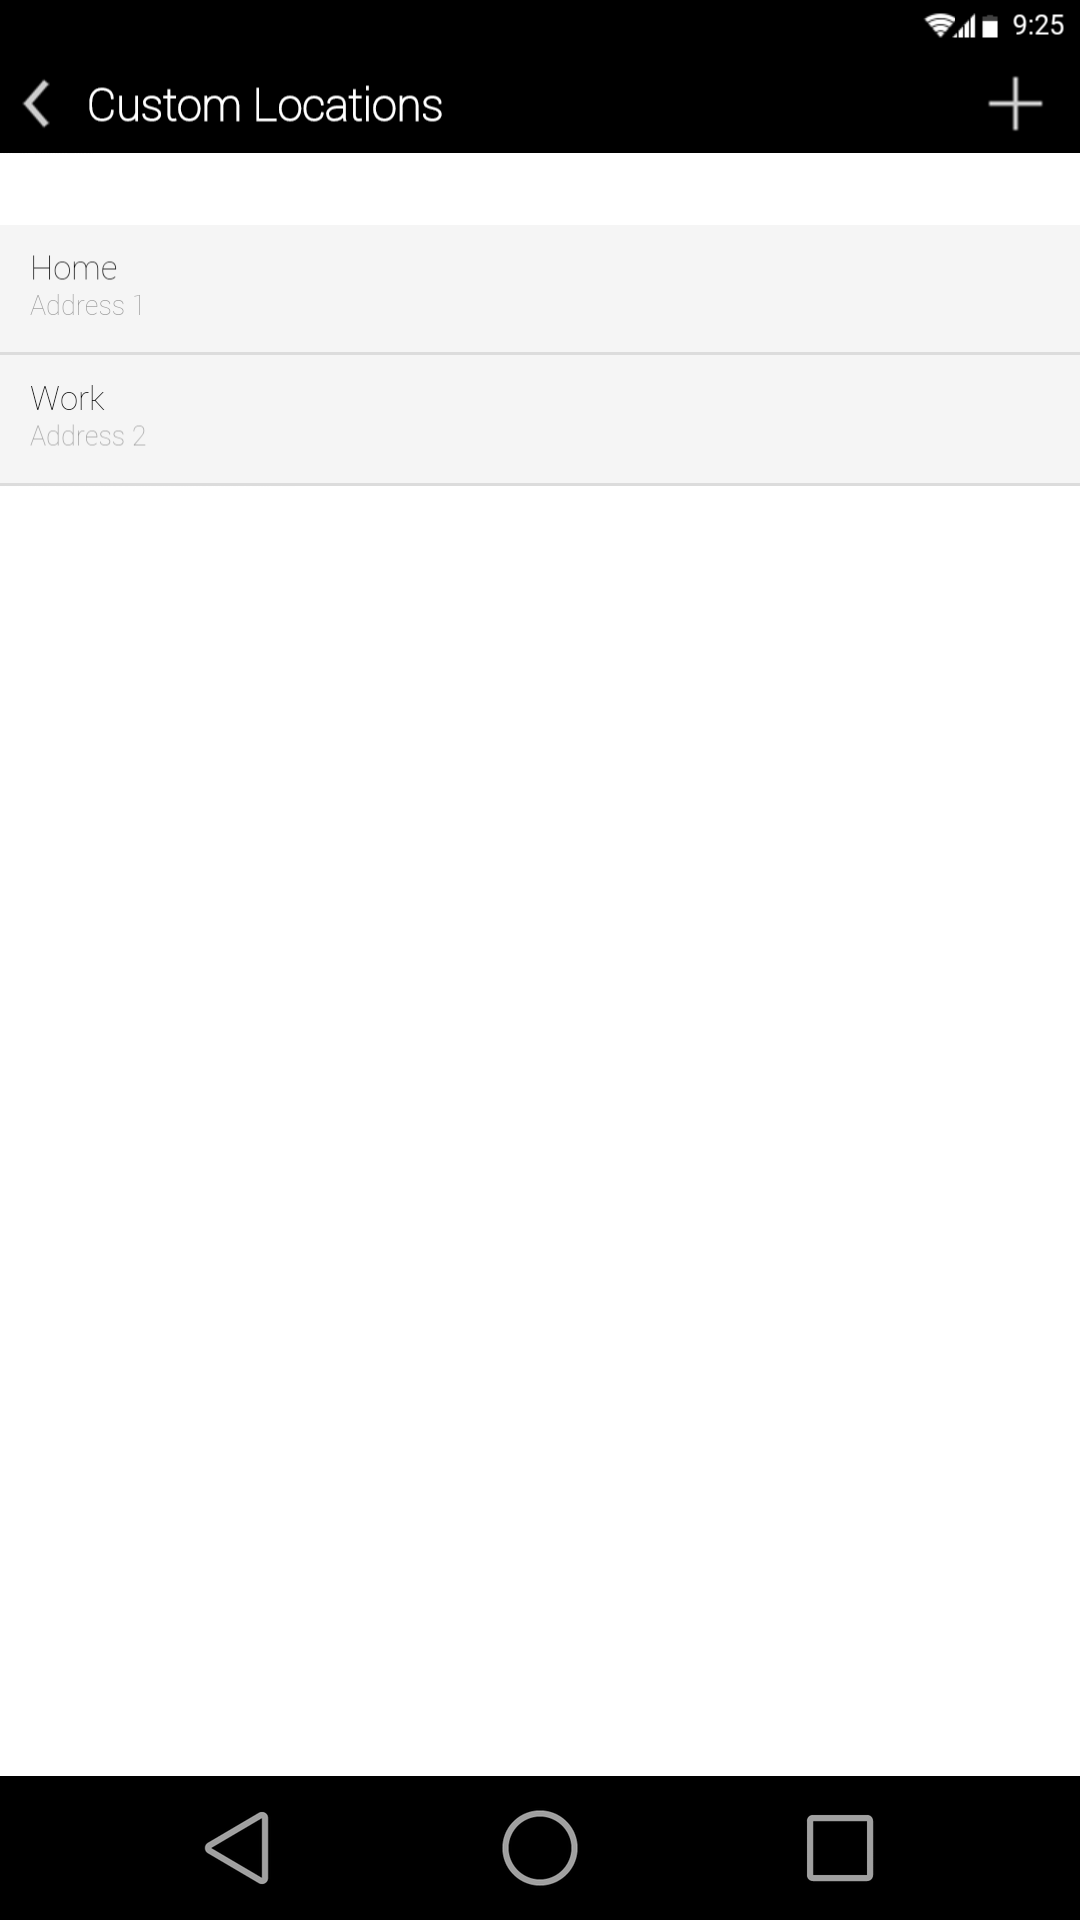
\includegraphics[width=5cm]{images/custom-list.png}}
	\caption{CUSTOM}
}
\end{figure}
\bigskip
\textbf{Description: }The user can select one of their previous custom locations
or press the \(+\) symbol to take them to add another custom location.

\textbf{Features: }Add new custom location (partial).

\begin{figure}[H]
\centering{
	\fbox{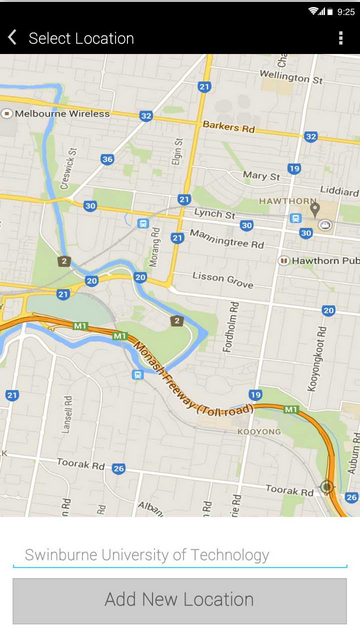
\includegraphics[width=5cm]{images/map.png}}
	\caption{MAP}
}
\end{figure}
\bigskip
\textbf{Description: }User can either pin a point on the map or search for a
location in the search bar. This will add it to the custom locations list and
allow them to see the sun times and weather.

\textbf{Features: }Add custom locations. Integrated into Google maps. View sun
rise / set times for various locations on a map.

\begin{figure}[H]
\centering{
	\fbox{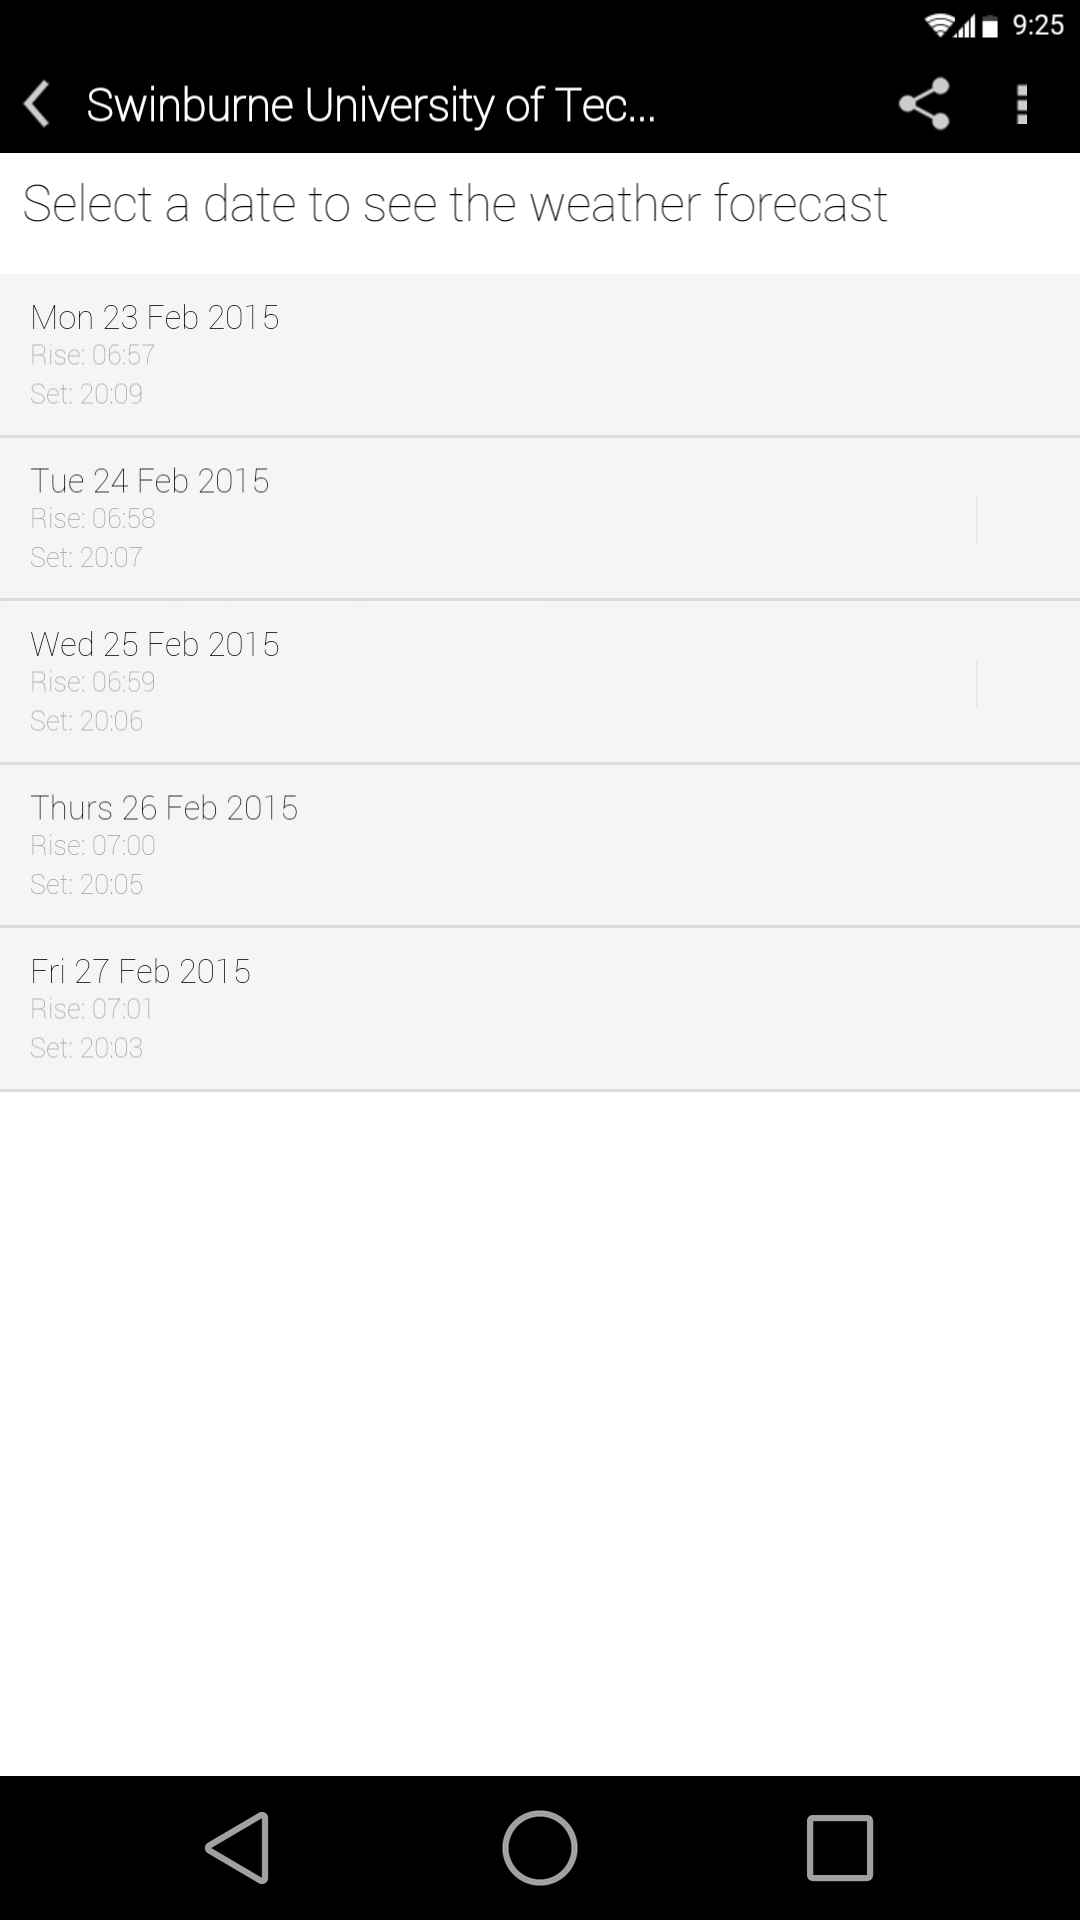
\includegraphics[width=5cm]{images/sun-range.png}}
	\caption{SUN-RANGE}
}
\end{figure}
\bigskip
\textbf{Description: }This screen shows the sun times for a range of dates which
was requested on the previous screen \textit{DATE-SELECT}. User can click on any
date and see the full \textit{WEATHER} screen as well.

\textbf{Features: }Generate table of sun rise/set times for a date range.

\subsubsection{User scenario validations}
\begin{enumerate}
	\item{Brad can enter the Wellington harbour into the app as a custom location.
	Once added Brad can select the dates he would like sun rise times for and view them.
	HOME $\rightarrow$ CUSTOM $\rightarrow$ MAP $\rightarrow$ CUSTOM $\rightarrow$ DATE-SELECT $\rightarrow$ SUN-WEATHER / SUN-RANGE}
	\item{Sachin can easily achieve this by adding each of the locations he will be
	and then generating sun rise and set times for the date range required. He can
	then easily share them by email with himself to print off.
	HOME $\rightarrow$ CUSTOM $\rightarrow$ MAP $\rightarrow$ CUSTOM $\rightarrow$ DATE-SELECT $\rightarrow$ SUN-RANGE $\rightarrow$ (Share button)}
	\item{Li can find Sydney as a preset location and select the date for tomorrow
	to see the sun rise time.
	HOME $\rightarrow$ PRESETS $\rightarrow$ DATE-SELECT $\rightarrow$ SUN-WEATHER}
	\item{Justin and Mary can select the current location option on the homescreen
	to get the data for their current GPS location and also share that with their
	friends.
	HOME $\rightarrow$ DATE-SELECT $\rightarrow$ SUN-WEATHER $\rightarrow$ (Share button)}
\end{enumerate}

\end{document}
